\chapter{Métodos Numéricos}\label{cap:metodos-numericos}
\graphicspath{{chapter-03/img-cap03/}}

Em todo caso de aplicação de um método numérico, deve-se iniciar pela modelagem matemática do problema. Desta forma, compreende-se como se encontra uma possível solução a partir das considerações necessárias para o problema. Após modelar o problema, faz-se necessário o uso de técnicas de discretização espaciais e temporais para transformar as equações diferenciais em equações algébricas.

As equações de Navier-Stokes podem ser escritas em variadas formas, a depender dos sistemas de coordenadas. Neste presente trabalho, as coordenadas cartesianas e ortogonais serão exploradas. Por necessidade da discretização, há alguns tipos de malhas que podem ser desenvolvidas: 

\begin{enumerate}
    \item Estruturadas: normalmente são produzidas através de uma mesma família de elementos (ex: formato quadrilátero numa malha 2D). A sua maior restrição é que normalmente se aplica estas malhas em geometria bastante simplificadas. Em malhas 3D, os erros se propagam em razão da dificuldade de controlar a distribuição de pontos;
    \item Estruturadas em blocos: há subdivisões do domínio para facilitar o refino somente onde é necessário. Contudo, há de se considerar os tratamentos nas interfaces dos subdomínios para manter a boa qualidade da malha. Em geometrias mais complexas, esta técnica costuma ter maior aplicação quando se deseja manter uma só família de elementos;
    \item Não-estruturadas: esse tipo de malha é a mais flexível para qualquer tipo de geometria. Na prática, os elementos podem ter várias formas, seja em malha 2D ou 3D. Para aplicações industriais, as malhas não-estruturadas são mais aplicadas, mesmo que haja uma perda de eficiência computacional, se comparadas com as malhas estruturadas.
\end{enumerate}

Sobre os métodos de solução, depende do problema. Seja um problema estacionário ou transiente, os problemas são altamente não-lineares, logo exige um processo iterativo para resolver. Em regra, o tipo de malha e o número de nós envolvidos é o que define a escolha pelo método mais eficiente. Por último, considera-se o critério de convergência, pois é com eles que se analisa as iterações para o método de solução escolhido. 

As mais importantes propriedades são consideradas a partir do que é proposto por \citeauthor{Ferziger&Peric2020}:

\begin{enumerate}
    \item Consistência: para o método ser considerado \textit{consistente}, o valor do erro de truncamento causado pela diferença entre a equação exata e a algébrica deve ser igual a zero. Para uma simulação ter consistência, é preciso se atentar com erros na mesma ordem de precisão, principalmente termos convectivos para altos números de Reynolds ou para os termos difusivos quando se tem baixos números de Reynolds. Contudo, essa propriedade não garante que a solução das equações discretas serão as soluções exatas no limite do intervalo de tempo. Para isso ocorrer, a solução deve ser \textit{estável}.
    \item Estabilidade: uma solução numérica é \textit{estável} quando os erros não se sobressaem ao longo das iterações e garante que a solução seja limitada na mesma ordem que a solução exata. Em suma, um método estável é aquele que não diverge.
    \item Convergência: um método é dito convergente quando a solução das equações discretas tendem à solução exata da equação diferencial quando o refino de malha reduz o espaçamento dos elementos a zero. Como é difícil verificar matematicamente se a solução convergiu, testes experimentais ou valores de referências são comparados com o que se obteve numericamente. Teste de independência de malha também costumam ser feitos para verificar se a solução também é estável e consistente.
    \item Conservação: como as equações a serem resolvidas são leis de conservação, para um volume de controle uma quantidade especificada saindo deste em regime estacionário e ausente de agentes externos significa que é igual ao valor de entrada neste mesmo volume.
    \item Limitado: as propriedades devem satisfazer suas próprias restrições. Propriedades escalares não-negativas (ex: densidade) devem resultar em valores positivos. Sem termos-fonte, propriedades como temperatura precisam se enquadrar entre os valores das condições de contorno.
    \item Realizável: o objetivo desta propriedade é garantir que as soluções sejam realistas, principalmente quando há fenômenos complexos, como a turbulência.;
    \item Precisão: como os métodos numéricos apenas oferecem soluções aproximadas, logo possui erros que se encaixam em um desses três perfis:
    \begin{enumerate}
        \item erros de modelo: diferença entre o escoamento simulado e a solução exata do modelo matemático. No caso de escoamentos turbulentos, o modelo pode ter assumido erros durante a derivação das equações de transporte. Pode acontecer quando há uma simplificação da geometria do domínio ou da condição de contorno. Por esta razão, é muito relevante ter acesso a valores de referência, seja de testes experimentais ou de soluções diretas de turbulência, etc.
        \item erros de discretização: diferença entre a solução exata das equações de conservação e a solução algébrica do sistema de equações obtida pela discretização dessas formulações. Com refino de malha, espera-se que esses erros diminuam.  
        \item erros de iteração: diferença entre a solução exata da solução do sistema algébrico e do processo iterativo. São também chamados de \textit{erros de convergência}.
    \end{enumerate}
\end{enumerate}

Como pré-requisitos para transformar as equações analíticas em algébricas, as técnicas de discretização mais aplicadas aos problemas de dinâmicas dos fluidos computacional são descritas a seguir \cite{Ferziger&Peric2020}.

\begin{enumerate}
    \item Diferenças Finitas: é o método mais antigo e simples para resolver equações diferenciais parciais (EDP). O ponto inicial é colocar as equações de conservação na forma diferencial, sendo o domínio da solução uma malha discretizada, onde cada nó representa os valores aproximados das funções discretas obtidas através das EDP. É mais aplicado em geometrias simples, onde a malha é estruturada. A maior desvantagem é que a conservação das propriedades não é garantida, exceto se houve um tratamento específico.
    \item Volumes Finitos: neste método a malha se divide em um número finito de volumes de controle (VC) de tal forma que as propriedades do fluido são calculadas para a superfície do VC através de interpolações nos nós. Esta técnica pode ser aplicada em qualquer tipo de malha, inclusive em geometrias complexas. Esta abordagem de discretização é conservativa por natureza, sendo uma razão pela qual as análises em CFD a tornam mais usual. Sua principal desvantagem é aplicar métodos acima de segunda ordem em malhas 3D, pois exige interpolação, diferenciação e integração.
    \item Elementos Finitos: apesar de haver uma similaridade com o método de volumes finitos, suas equações são multiplicadas por funções peso antes de serem integradas num domínio. No casos mais simples, a função é aproximada por uma função linear. O resultado desta técnica é gerar um sistema de equações algébricas não-lineares. É ótimo para lidar com geometrias arbitrárias. Sua principal deficiência está na resolução de malhas não-estruturadas, pois a construção de matrizes do sistema não-linear não se forma a permitir aplicações de técnicas para solucionar.
\end{enumerate}

\section{Método dos Volumes Finitos}

Supondo que $\phi$ seja uma variável referente a uma propriedade do fluido, o método de volumes finitos (MVF) se utiliza da forma integral da equação de transporte, como é apresentado na equação \ref{eq:volumes-finitos}.

\begin{equation}
    \label{eq:volumes-finitos}
    \int_{\forall} \frac{\partial \rho\phi}{\partial t} \hspace{0.5pt} d\forall + \int_{A} \rho\phi\boldsymbol{u}\cdot\boldsymbol{n}\hspace{0.5pt} dA = \int_{A} \Gamma_{\phi}\nabla\phi\cdot\boldsymbol{n}\hspace{0.5pt} dA + \int_{\forall} S_{\phi}\hspace{0.5pt} d\forall
\end{equation}

Os dois termos à esquerda se referem ao termo transiente por unidade de volume e o termo convectivo, respectivamente. Enquanto isso, do outro lado da equação tem-se, seguindo da esquerda para a direita, o termo difusivo e o termo-fonte. As notações em negrito são vetores. O domínio da solução é subdividido em vários volumes de controle dentro de uma malha. Acerca dos sistemas de coordenadas, este trabalho utilizará o sistema cartesiano. A abordagem de volumes finitos aplicará os resultados das integrações das equações de conservação para o centro dos volumes de controle, embora haja outras variantes. O somatório dos resultados será o valor global das equações e é por isso que o MVF se apresenta como uma técnica vantajosa para simulações CFD.

A discretização geral das equações de conservação \ref{eq:volumes-finitos} se resume a equação \ref{eq:volumes-finitos-discreta}:

\begin{equation}
    \label{eq:volumes-finitos-discreta}
    \frac{\partial \rho\phi}{\partial t}\forall + \sum_{f}^{N_{faces}}\rho_{f}\phi_{f}\boldsymbol{u}_f\boldsymbol{A}_{f} = \sum_{f}^{N_{faces}}\Gamma_{\phi}\nabla\phi_{f}\boldsymbol{A}_{f} + S_{\phi}\forall
\end{equation}
%
onde $N_{faces}$ é igual ao número de faces envolvendo a célula; $\phi_f$, o valor de $\phi$ convectada através da face f; $\rho_f\boldsymbol{u}_f\textbf{A}_f$ é o fluxo de massa através da face; $\textbf{A}_f$, o vetor da área da face; $\nabla\phi_f$ equivale ao gradiente de $\phi$ na face f e $\forall$ é o volume de controle arbitrário. A forma linearizada da equação \ref{eq:volumes-finitos-discreta} é apresentada em \ref{eq:forma-linear-mvf}:

\begin{equation}
    \label{eq:forma-linear-mvf}
    a_{p}\phi = \sum_{nb}a_{nb}\phi_{nb} + b
\end{equation}
%
onde o subscrito $nb$ se refere às células vizinhas, enquanto que $a_{p}$ e $a_{nb}$ são coeficientes linearizados de $\phi$ e $\phi_{nb}$. O número de vizinhos depende da topologia da malha, mas o resultado é um sistema de equações com matriz de coeficientes esparsos.

\subsection{Algoritmos de resolução de escoamentos}

Há dois tipos principais de algoritmos para resolver as equações de transporte de continuidade, momentum e energia:

\begin{enumerate}
    \item \textit{Pressure-based}: costumam atender os casos de baixas velocidades e em regime incompressível.
    \item \textit{Density-based}: costumam ser usados em escoamentos compressíveis a altas velocidades.
\end{enumerate}

Apesar de suas aplicações usuais, os métodos já foram reformulados para atender uma variedade de condições além do que foram propostos a fazer. Em ambos os casos, o campo de velocidade é obtido pela equação de momentum, enquanto que no algoritmo \textit{density-based} resolve a densidade pela conservação de massa e o campo de pressão a partir de uma equação de estado. Por outro lado, na abordagem \textit{pressure-based}, o campo de pressão é resolvido por uma equação para a pressão ou o ajuste desta propriedade que é obtida pela manipulação das equações de continuidade e momentum.

Seja qual for o método, serão resolvidas as equações de transporte para a continuidade e momentum, assim como para a energia, turbulência e espécies químicas, se houver necessidade. A maneira que as equações de governo são linearizadas podem resultar numa forma “implícita” ou “explícita”. Tal explicação é demonstrada a seguir:

\begin{enumerate}
    \item Implícita: para uma dada variável, o valor a descobrir em cada volume de controle $\forall$ é computado usando uma relação que inclui os valores existentes e desconhecidos das células vizinhas. Portanto, cada valor desejado aparecerá em mais de uma equação algébrica, onde essas equações devem ser resolvidas simultaneamente para obter o valores desconhecidos.
    \item Explícita: para uma dada variável, o valor a descobrir lume de controle $\forall$ é computado usando uma relação que inclui só os valores existentes das células vizinhas. Portanto, cada valor desejado aparecerá em apenas uma equação algébrica, onde essas equações são resolvidas sequencialmente para obter o valores desconhecidos. 
\end{enumerate}

\subsubsection{Algoritmo \textit{Pressure-Based}}

O campo de velocidade é calculado após resolver uma equação para o campo de pressão (ou o ajuste da pressão). Essa equação é derivada das conservações de massa e momentum, onde o campo de velocidade também satisfaz a continuidade \cite{Chorin68}. Por ser um sistema altamente não-linear e acoplado, necessita-se de um processo iterativo até atingir a convergência da solução. Há duas possibilidades de algoritmos \textit{pressure-based}, como mostra a Figura \ref{flux:pressure-based}. 

\begin{figure}[!ht]
\centering
\tikzset{every picture/.style={line width=0.75pt}} %set default line width to 0.75pt        

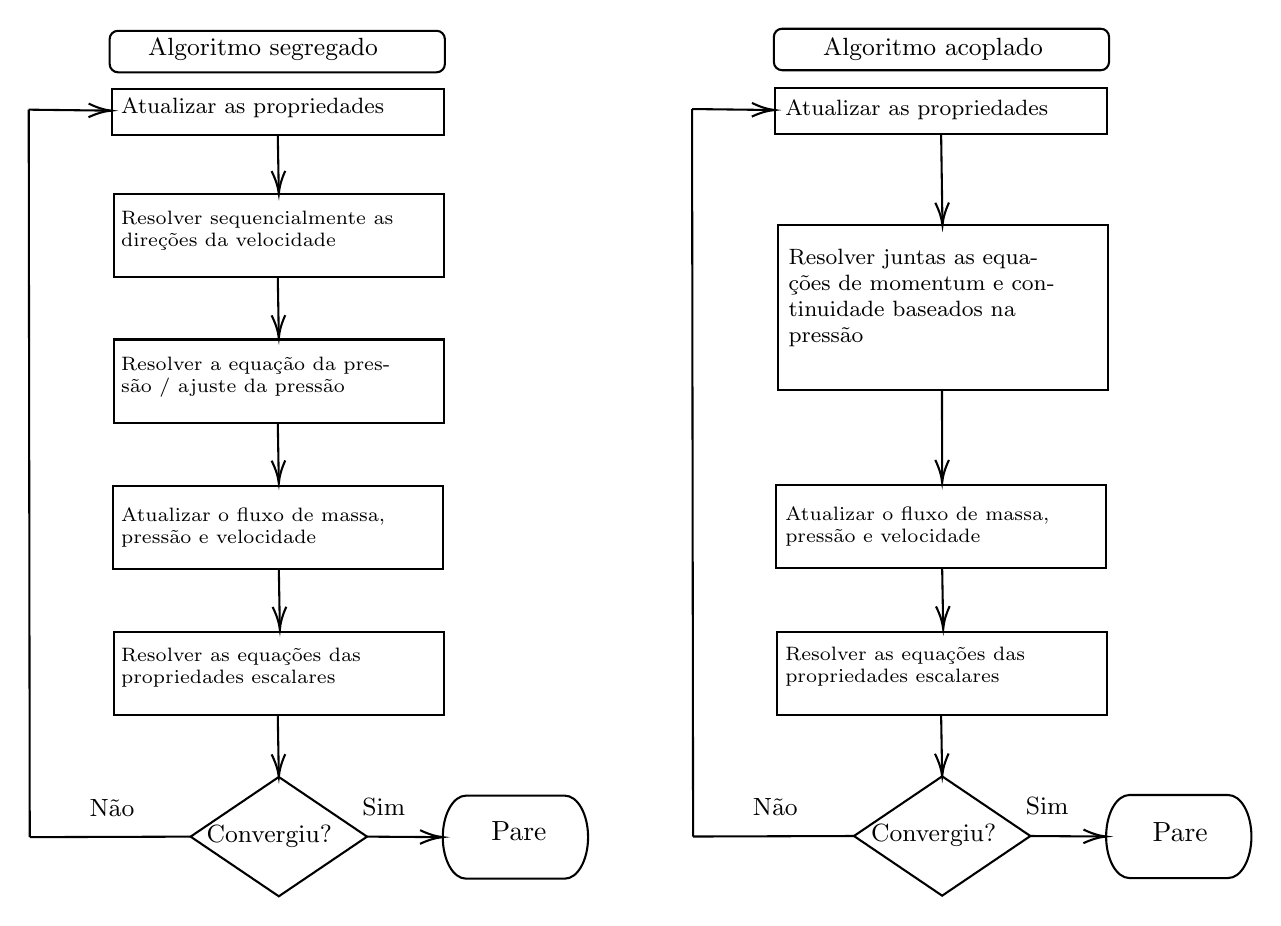
\begin{tikzpicture}[x=0.75pt,y=0.75pt,yscale=-1,xscale=1]
%uncomment if require: \path (0,476); %set diagram left start at 0, and has height of 476

%Shape: Rectangle [id:dp5456242229572967] 
\draw   (80,54.75) -- (240,54.75) -- (240,76.75) -- (80,76.75) -- cycle ;
%Shape: Rectangle [id:dp5146003696778889] 
\draw   (81,105.5) -- (240,105.5) -- (240,145.5) -- (81,145.5) -- cycle ;
%Straight Lines [id:da7993405819141195] 
\draw    (160,77) -- (160.46,103.25) ;
\draw [shift={(160.5,105.25)}, rotate = 268.99] [color={rgb, 255:red, 0; green, 0; blue, 0 }  ][line width=0.75]    (10.93,-3.29) .. controls (6.95,-1.4) and (3.31,-0.3) .. (0,0) .. controls (3.31,0.3) and (6.95,1.4) .. (10.93,3.29)   ;
%Straight Lines [id:da06909790258431547] 
\draw    (160,145.5) -- (160.47,172.75) ;
\draw [shift={(160.5,174.75)}, rotate = 269.02] [color={rgb, 255:red, 0; green, 0; blue, 0 }  ][line width=0.75]    (10.93,-3.29) .. controls (6.95,-1.4) and (3.31,-0.3) .. (0,0) .. controls (3.31,0.3) and (6.95,1.4) .. (10.93,3.29)   ;
%Shape: Rectangle [id:dp5311740933172808] 
\draw   (81,175.5) -- (240,175.5) -- (240,215.5) -- (81,215.5) -- cycle ;
%Straight Lines [id:da5901369105046621] 
\draw    (160,215.5) -- (160.47,242.75) ;
\draw [shift={(160.5,244.75)}, rotate = 269.02] [color={rgb, 255:red, 0; green, 0; blue, 0 }  ][line width=0.75]    (10.93,-3.29) .. controls (6.95,-1.4) and (3.31,-0.3) .. (0,0) .. controls (3.31,0.3) and (6.95,1.4) .. (10.93,3.29)   ;
%Shape: Rectangle [id:dp4189524190256626] 
\draw   (80.5,246) -- (239.5,246) -- (239.5,286) -- (80.5,286) -- cycle ;
%Straight Lines [id:da7692950512064372] 
\draw    (160.5,286) -- (160.97,313.25) ;
\draw [shift={(161,315.25)}, rotate = 269.02] [color={rgb, 255:red, 0; green, 0; blue, 0 }  ][line width=0.75]    (10.93,-3.29) .. controls (6.95,-1.4) and (3.31,-0.3) .. (0,0) .. controls (3.31,0.3) and (6.95,1.4) .. (10.93,3.29)   ;
%Shape: Rectangle [id:dp5046834721515459] 
\draw   (81,316.5) -- (240,316.5) -- (240,356.5) -- (81,356.5) -- cycle ;
%Flowchart: Decision [id:dp6914527803231723] 
\draw   (160.5,386.25) -- (203,415) -- (160.5,443.75) -- (118,415) -- cycle ;
%Straight Lines [id:da641257311737564] 
\draw    (160,357) -- (160.47,384.25) ;
\draw [shift={(160.5,386.25)}, rotate = 269.02] [color={rgb, 255:red, 0; green, 0; blue, 0 }  ][line width=0.75]    (10.93,-3.29) .. controls (6.95,-1.4) and (3.31,-0.3) .. (0,0) .. controls (3.31,0.3) and (6.95,1.4) .. (10.93,3.29)   ;
%Straight Lines [id:da970365971837885] 
\draw    (203,415) -- (237.5,415.24) ;
\draw [shift={(239.5,415.25)}, rotate = 180.39] [color={rgb, 255:red, 0; green, 0; blue, 0 }  ][line width=0.75]    (10.93,-3.29) .. controls (6.95,-1.4) and (3.31,-0.3) .. (0,0) .. controls (3.31,0.3) and (6.95,1.4) .. (10.93,3.29)   ;
%Flowchart: Terminator [id:dp947666633166445] 
\draw   (250.7,395.25) -- (298.3,395.25) .. controls (304.49,395.25) and (309.5,404.2) .. (309.5,415.25) .. controls (309.5,426.3) and (304.49,435.25) .. (298.3,435.25) -- (250.7,435.25) .. controls (244.51,435.25) and (239.5,426.3) .. (239.5,415.25) .. controls (239.5,404.2) and (244.51,395.25) .. (250.7,395.25) -- cycle ;
%Straight Lines [id:da7859174596491716] 
\draw    (40,64.75) -- (40.5,415.25) ;
%Straight Lines [id:da7515603235516235] 
\draw    (118,415) -- (40.5,415.25) ;
%Straight Lines [id:da6386965161765668] 
\draw    (40,64.75) -- (77.77,65.21) ;
\draw [shift={(79.77,65.23)}, rotate = 180.69] [color={rgb, 255:red, 0; green, 0; blue, 0 }  ][line width=0.75]    (10.93,-3.29) .. controls (6.95,-1.4) and (3.31,-0.3) .. (0,0) .. controls (3.31,0.3) and (6.95,1.4) .. (10.93,3.29)   ;
%Shape: Rectangle [id:dp6955840613043904] 
\draw   (399.6,54.45) -- (559.6,54.45) -- (559.6,76.45) -- (399.6,76.45) -- cycle ;
%Shape: Rectangle [id:dp2470197636955902] 
\draw   (401.1,120.5) -- (560.1,120.5) -- (560.1,200) -- (401.1,200) -- cycle ;
%Straight Lines [id:da36804399782889763] 
\draw    (479.6,76.7) -- (480.22,118.5) ;
\draw [shift={(480.25,120.5)}, rotate = 269.15] [color={rgb, 255:red, 0; green, 0; blue, 0 }  ][line width=0.75]    (10.93,-3.29) .. controls (6.95,-1.4) and (3.31,-0.3) .. (0,0) .. controls (3.31,0.3) and (6.95,1.4) .. (10.93,3.29)   ;
%Straight Lines [id:da9013024578546147] 
\draw    (480,199.75) -- (480.1,242.45) ;
\draw [shift={(480.1,244.45)}, rotate = 269.87] [color={rgb, 255:red, 0; green, 0; blue, 0 }  ][line width=0.75]    (10.93,-3.29) .. controls (6.95,-1.4) and (3.31,-0.3) .. (0,0) .. controls (3.31,0.3) and (6.95,1.4) .. (10.93,3.29)   ;
%Shape: Rectangle [id:dp4764395574363469] 
\draw   (400.1,245.7) -- (559.1,245.7) -- (559.1,285.7) -- (400.1,285.7) -- cycle ;
%Straight Lines [id:da1290244750194034] 
\draw    (480.1,285.7) -- (480.57,312.95) ;
\draw [shift={(480.6,314.95)}, rotate = 269.02] [color={rgb, 255:red, 0; green, 0; blue, 0 }  ][line width=0.75]    (10.93,-3.29) .. controls (6.95,-1.4) and (3.31,-0.3) .. (0,0) .. controls (3.31,0.3) and (6.95,1.4) .. (10.93,3.29)   ;
%Shape: Rectangle [id:dp6352478239859609] 
\draw   (400.6,316.2) -- (559.6,316.2) -- (559.6,356.2) -- (400.6,356.2) -- cycle ;
%Flowchart: Decision [id:dp17744394343128667] 
\draw   (480.1,385.95) -- (522.6,414.7) -- (480.1,443.45) -- (437.6,414.7) -- cycle ;
%Straight Lines [id:da885342291248687] 
\draw    (479.6,356.7) -- (480.07,383.95) ;
\draw [shift={(480.1,385.95)}, rotate = 269.02] [color={rgb, 255:red, 0; green, 0; blue, 0 }  ][line width=0.75]    (10.93,-3.29) .. controls (6.95,-1.4) and (3.31,-0.3) .. (0,0) .. controls (3.31,0.3) and (6.95,1.4) .. (10.93,3.29)   ;
%Straight Lines [id:da9995731339683702] 
\draw    (522.6,414.7) -- (557.1,414.94) ;
\draw [shift={(559.1,414.95)}, rotate = 180.39] [color={rgb, 255:red, 0; green, 0; blue, 0 }  ][line width=0.75]    (10.93,-3.29) .. controls (6.95,-1.4) and (3.31,-0.3) .. (0,0) .. controls (3.31,0.3) and (6.95,1.4) .. (10.93,3.29)   ;
%Flowchart: Terminator [id:dp03700567233492813] 
\draw   (570.3,394.95) -- (617.9,394.95) .. controls (624.09,394.95) and (629.1,403.9) .. (629.1,414.95) .. controls (629.1,426) and (624.09,434.95) .. (617.9,434.95) -- (570.3,434.95) .. controls (564.11,434.95) and (559.1,426) .. (559.1,414.95) .. controls (559.1,403.9) and (564.11,394.95) .. (570.3,394.95) -- cycle ;
%Straight Lines [id:da714897424737142] 
\draw    (359.6,64.45) -- (360.1,414.95) ;
%Straight Lines [id:da5698935015214337] 
\draw    (437.6,414.7) -- (360.1,414.95) ;
%Straight Lines [id:da037788770764761725] 
\draw    (359.6,64.45) -- (397.37,64.91) ;
\draw [shift={(399.37,64.93)}, rotate = 180.69] [color={rgb, 255:red, 0; green, 0; blue, 0 }  ][line width=0.75]    (10.93,-3.29) .. controls (6.95,-1.4) and (3.31,-0.3) .. (0,0) .. controls (3.31,0.3) and (6.95,1.4) .. (10.93,3.29)   ;
%Rounded Rect [id:dp7855365314760501] 
\draw   (79,30.75) .. controls (79,28.54) and (80.79,26.75) .. (83,26.75) -- (236.5,26.75) .. controls (238.71,26.75) and (240.5,28.54) .. (240.5,30.75) -- (240.5,42.75) .. controls (240.5,44.96) and (238.71,46.75) .. (236.5,46.75) -- (83,46.75) .. controls (80.79,46.75) and (79,44.96) .. (79,42.75) -- cycle ;
%Rounded Rect [id:dp7552054721421797] 
\draw   (399,29.75) .. controls (399,27.54) and (400.79,25.75) .. (403,25.75) -- (556.5,25.75) .. controls (558.71,25.75) and (560.5,27.54) .. (560.5,29.75) -- (560.5,41.75) .. controls (560.5,43.96) and (558.71,45.75) .. (556.5,45.75) -- (403,45.75) .. controls (400.79,45.75) and (399,43.96) .. (399,41.75) -- cycle ;

% Text Node
\draw (83,57.5) node [anchor=north west][inner sep=0.75pt]  [font=\footnotesize] [align=left] {Atualizar as propriedades};
% Text Node
\draw (83,112) node [anchor=north west][inner sep=0.75pt]  [font=\scriptsize] [align=left] {Resolver sequencialmente as\\direções da velocidade};
% Text Node
\draw (83,182.5) node [anchor=north west][inner sep=0.75pt]  [font=\scriptsize] [align=left] {Resolver a equação da pres-\\são / ajuste da pressão};
% Text Node
\draw (83,255) node [anchor=north west][inner sep=0.75pt]  [font=\scriptsize] [align=left] {Atualizar o fluxo de massa, \\pressão e velocidade};
% Text Node
\draw (83,322.5) node [anchor=north west][inner sep=0.75pt]  [font=\scriptsize] [align=left] {Resolver as equações das \\propriedades escalares};
% Text Node
\draw (124.25,408) node [anchor=north west][inner sep=0.75pt]  [font=\small] [align=left] {Convergiu?};
% Text Node
\draw (258.5,406.25) node [anchor=north west][inner sep=0.75pt]  [font=\normalsize] [align=left] {\begin{minipage}[lt]{24.27pt}\setlength\topsep{0pt}
\begin{center}
Pare
\end{center}

\end{minipage}};
% Text Node
\draw (86.75,401) node  [font=\small] [align=left] {\begin{minipage}[lt]{26.18pt}\setlength\topsep{0pt}
Não
\end{minipage}};
% Text Node
\draw (218.25,400.5) node  [font=\small] [align=left] {\begin{minipage}[lt]{26.18pt}\setlength\topsep{0pt}
Sim
\end{minipage}};
% Text Node
\draw (403,58.7) node [anchor=north west][inner sep=0.75pt]  [font=\footnotesize] [align=left] {Atualizar as propriedades};
% Text Node
\draw (403,254.7) node [anchor=north west][inner sep=0.75pt]  [font=\scriptsize] [align=left] {Atualizar o fluxo de massa,\\pressão e velocidade};
% Text Node
\draw (403,322.2) node [anchor=north west][inner sep=0.75pt]  [font=\scriptsize] [align=left] {Resolver as equações das\\propriedades escalares};
% Text Node
\draw (444.35,407.45) node [anchor=north west][inner sep=0.75pt]  [font=\small] [align=left] {Convergiu?};
% Text Node
\draw (577.1,406.7) node [anchor=north west][inner sep=0.75pt]  [font=\normalsize] [align=left] {\begin{minipage}[lt]{24.27pt}\setlength\topsep{0pt}
\begin{center}
Pare
\end{center}

\end{minipage}};
% Text Node
\draw (406.35,400.7) node  [font=\small] [align=left] {\begin{minipage}[lt]{26.18pt}\setlength\topsep{0pt}
Não
\end{minipage}};
% Text Node
\draw (537.85,400.2) node  [font=\small] [align=left] {\begin{minipage}[lt]{26.18pt}\setlength\topsep{0pt}
Sim
\end{minipage}};
% Text Node
\draw (404.6,130.25) node [anchor=north west][inner sep=0.75pt]  [font=\footnotesize] [align=left] {Resolver juntas as equa-\\ções de momentum e con-\\tinuidade baseados na\\pressão};
% Text Node
\draw (96,28.75) node [anchor=north west][inner sep=0.75pt]  [font=\small] [align=left] {Algoritmo segregado};
% Text Node
\draw (421.25,28.75) node [anchor=north west][inner sep=0.75pt]  [font=\small] [align=left] {Algoritmo acoplado};\
\end{tikzpicture}
\caption[Fluxogramas para algoritmo \textit{pressure-based} segregado e acoplado.]{Fluxogramas para algoritmo \textit{pressure-based} segregado e acoplado \cite{fluent2021ansys}.}
\label{flux:pressure-based}
\end{figure}

Ambos os casos tem prós e contras, quando analisadas as convergências das soluções e o uso de memória computacional. A \autoref{tab:esquema-comparacao-segregado-acoplado} resume as diferenças entre os tipos de algoritmos.

\begin{table}[ht]
\centering
\vspace{0.5cm}
\caption[Comparações entre os algoritmos segregados e acoplados.]{Comparações entre os algoritmos segregados e acoplados.}
\begin{tabular}[c]{c|c|c}
Tipo de algoritmo & Convergência da solução & Uso de memória \\
\hline
Segregado & Baixo & Baixo \\
Acoplado & Baixo & Alto
\end{tabular}
\label{tab:esquema-comparacao-segregado-acoplado}
\end{table}

As comparações da \autoref{tab:esquema-comparacao-segregado-acoplado} são baseadas nos desempenhos dos próprios algoritmos.

\subsubsection{Algoritmo \textit{Density-Based}}

Esse algoritmo busca resolver as equações de transporte para a conservação da massa, momentum e energia simultaneamente \cite{Weiss1995PreconditioningAT, Weiss1997IMPLICITSO, Weiss1999ImplicitSO}. As equações adicionais de turbulência e espécies químicas (se houver) são resolvidas sequencialmente. Assim como o método \textit{pressure-based}, há a necessidade de se resolver iterativamente até atingir a convergência da solução. Na Figura \ref{fig:density-based} é apresentado o fluxograma para a compreensão do método \cite{fluent2021ansys}.

\begin{figure}[!ht]
    \centering

\tikzset{every picture/.style={line width=0.75pt}} %set default line width to 0.75pt        

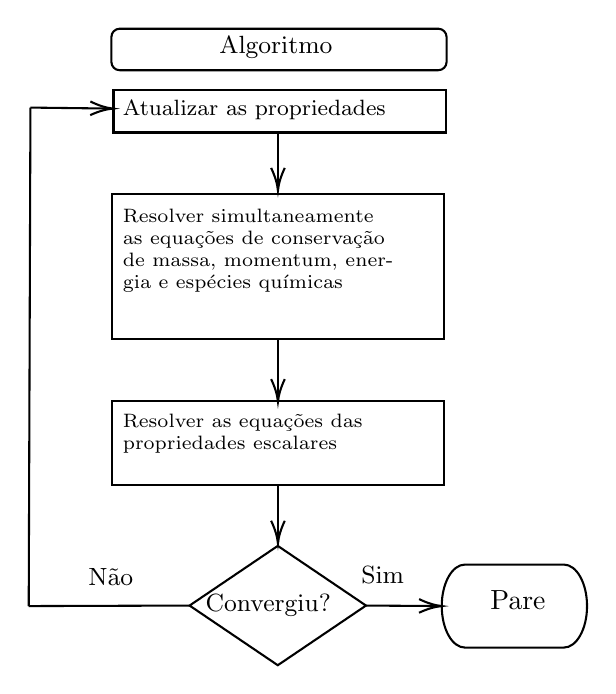
\begin{tikzpicture}[x=0.75pt,y=0.75pt,yscale=-1,xscale=1]
%uncomment if require: \path (0,476); %set diagram left start at 0, and has height of 476

%Shape: Rectangle [id:dp5456242229572967] 
\draw  [line width=0.75]  (231,60.25) -- (391,60.25) -- (391,80.75) -- (231,80.75) -- cycle ;
%Shape: Rectangle [id:dp5146003696778889] 
\draw  [line width=0.75]  (230.5,110.25) -- (390.25,110.25) -- (390.25,180.25) -- (230.5,180.25) -- cycle ;
%Shape: Rectangle [id:dp5046834721515459] 
\draw  [line width=0.75]  (230.5,210.25) -- (390.33,210.25) -- (390.33,250.5) -- (230.5,250.5) -- cycle ;
%Flowchart: Decision [id:dp6914527803231723] 
\draw  [line width=0.75]  (310.17,279.92) -- (352.67,308.67) -- (310.17,337.42) -- (267.67,308.67) -- cycle ;
%Straight Lines [id:da970365971837885] 
\draw [line width=0.75]    (352.67,308.67) -- (387.17,308.9) ;
\draw [shift={(389.17,308.92)}, rotate = 180.39] [color={rgb, 255:red, 0; green, 0; blue, 0 }  ][line width=0.75]    (10.93,-3.29) .. controls (6.95,-1.4) and (3.31,-0.3) .. (0,0) .. controls (3.31,0.3) and (6.95,1.4) .. (10.93,3.29)   ;
%Flowchart: Terminator [id:dp947666633166445] 
\draw  [line width=0.75]  (400.37,288.92) -- (447.97,288.92) .. controls (454.15,288.92) and (459.17,297.87) .. (459.17,308.92) .. controls (459.17,319.96) and (454.15,328.92) .. (447.97,328.92) -- (400.37,328.92) .. controls (394.18,328.92) and (389.17,319.96) .. (389.17,308.92) .. controls (389.17,297.87) and (394.18,288.92) .. (400.37,288.92) -- cycle ;
%Straight Lines [id:da7515603235516235] 
\draw [line width=0.75]    (267.67,308.67) -- (190.17,308.92) ;
%Straight Lines [id:da6386965161765668] 
\draw [line width=0.75]    (191,68.75) -- (228.77,69.21) ;
\draw [shift={(230.77,69.23)}, rotate = 180.69] [color={rgb, 255:red, 0; green, 0; blue, 0 }  ][line width=0.75]    (10.93,-3.29) .. controls (6.95,-1.4) and (3.31,-0.3) .. (0,0) .. controls (3.31,0.3) and (6.95,1.4) .. (10.93,3.29)   ;
%Rounded Rect [id:dp7855365314760501] 
\draw  [line width=0.75]  (230,34.75) .. controls (230,32.54) and (231.79,30.75) .. (234,30.75) -- (387.5,30.75) .. controls (389.71,30.75) and (391.5,32.54) .. (391.5,34.75) -- (391.5,46.75) .. controls (391.5,48.96) and (389.71,50.75) .. (387.5,50.75) -- (234,50.75) .. controls (231.79,50.75) and (230,48.96) .. (230,46.75) -- cycle ;
%Straight Lines [id:da9465483108271935] 
\draw    (310.25,80.75) -- (310.25,106.75) ;
\draw [shift={(310.25,108.75)}, rotate = 270] [color={rgb, 255:red, 0; green, 0; blue, 0 }  ][line width=0.75]    (10.93,-3.29) .. controls (6.95,-1.4) and (3.31,-0.3) .. (0,0) .. controls (3.31,0.3) and (6.95,1.4) .. (10.93,3.29)   ;
%Straight Lines [id:da3995043167173449] 
\draw    (310.25,180) -- (310.25,208.5) ;
\draw [shift={(310.25,210.5)}, rotate = 270] [color={rgb, 255:red, 0; green, 0; blue, 0 }  ][line width=0.75]    (10.93,-3.29) .. controls (6.95,-1.4) and (3.31,-0.3) .. (0,0) .. controls (3.31,0.3) and (6.95,1.4) .. (10.93,3.29)   ;
%Straight Lines [id:da04251926302512321] 
\draw    (310.25,250.75) -- (310.25,276.75) ;
\draw [shift={(310.25,278.75)}, rotate = 270] [color={rgb, 255:red, 0; green, 0; blue, 0 }  ][line width=0.75]    (10.93,-3.29) .. controls (6.95,-1.4) and (3.31,-0.3) .. (0,0) .. controls (3.31,0.3) and (6.95,1.4) .. (10.93,3.29)   ;
%Straight Lines [id:da9763303419571623] 
\draw    (191,68.75) -- (190.17,308.92) ;

% Text Node
\draw (234,63.5) node [anchor=north west][inner sep=0.75pt]  [font=\footnotesize] [align=left] {Atualizar as propriedades};
% Text Node
\draw (234,116) node [anchor=north west][inner sep=0.75pt]  [font=\scriptsize] [align=left] {Resolver simultaneamente\\as equações de conservação \\de massa, momentum, ener-\\gia e espécies químicas};
% Text Node
\draw (234,214.92) node [anchor=north west][inner sep=0.75pt]  [font=\scriptsize] [align=left] {Resolver as equações das\\propriedades escalares};
% Text Node
\draw (273.92,301.67) node [anchor=north west][inner sep=0.75pt]  [font=\small] [align=left] {Convergiu?};
% Text Node
\draw (408.17,299.92) node [anchor=north west][inner sep=0.75pt]  [font=\normalsize] [align=left] {\begin{minipage}[lt]{24.27pt}\setlength\topsep{0pt}
\begin{center}
Pare
\end{center}

\end{minipage}};
% Text Node
\draw (236.42,294.67) node  [font=\small] [align=left] {\begin{minipage}[lt]{26.18pt}\setlength\topsep{0pt}
Não
\end{minipage}};
% Text Node
\draw (367.92,294.17) node  [font=\small] [align=left] {\begin{minipage}[lt]{26.18pt}\setlength\topsep{0pt}
Sim
\end{minipage}};
% Text Node
\draw (280.5,32.75) node [anchor=north west][inner sep=0.75pt]  [font=\small] [align=left] {Algoritmo};

\end{tikzpicture}
\caption[Fluxograma para algoritmo \textit{density-based}]{Fluxograma para algoritmo \textit{density-based} \cite{fluent2021ansys}.}
\label{fig:density-based}
\end{figure}

\subsection{Discretização espacial}

Assumindo que se trata de um problema em regime estacionário, o termo $\frac{\partial \rho\phi}{\partial t}\forall$ pode ser desconsiderado da equação \ref{eq:volumes-finitos}, resultando na equação \ref{eq:volumes-finitos-estacionaria}:

\begin{equation}
    \label{eq:volumes-finitos-estacionaria}
    \int_{A} \rho\phi\boldsymbol{u}\cdot\boldsymbol{n}\hspace{0.5pt} dA = \int_{A} \Gamma_{\phi}\nabla\phi\cdot\boldsymbol{n}\hspace{0.5pt} dA + \int_{\forall} S_{\phi}\hspace{0.5pt} d\forall
\end{equation}

Os valores discretos de $\phi$ são obtidos no centros dos volumes de controle, mas os valores referentes às faces de $\phi$ são interpolados através dos valores centrais dos volumes de controle \cite{Rezende2009}. Os seguintes esquemas de discretização espacial serão tratados: diferenças centrais; \textit{upwind} de 1ª ordem e 2ª ordem e QUICK.

\subsubsection{Esquema de diferenças centrais}

O valor da variável na face do volume de controle $\phi_{f}$ é calculado da seguinte forma no esquema de diferenças centrais (CDS), conforme equação \ref{eq:esquema-CDS} \cite{Rezende2009}.

\begin{equation}
    \label{eq:esquema-CDS}
    \phi_f = \frac{1}{2}\left(\phi_0+\phi_1\right)+\frac{1}{2}\left(\nabla\phi_0\cdot\overrightarrow{r_0}+\nabla\phi_1\cdot\overrightarrow{r_1}\right)
\end{equation}

sendo 0 e 1 os índices das células representadas na Figura \ref{fig:volume-ANSYS-2021R2}, sendo $\overrightarrow{r}$ o vetor deslocamento que liga o centro da célula a montante à face do volume de controle. A Figura \ref{fig:volume-ANSYS-2021R2} ilustra a discretização de uma célula triangular bidimensional como exemplo de volume de controle \cite{fluent2021ansys}.

\begin{figure}[!ht] 
	\centering
	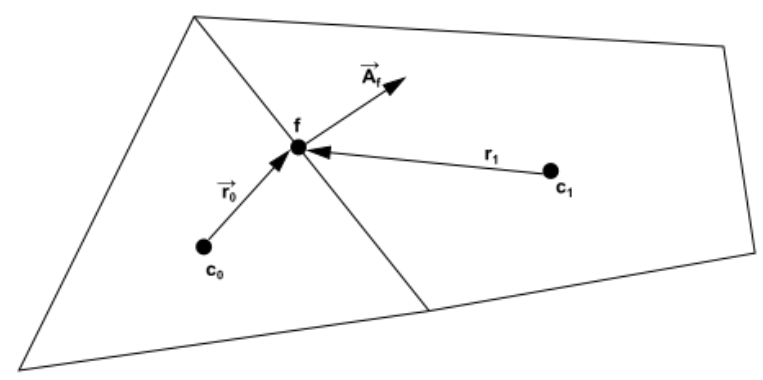
\includegraphics[width=0.5\textwidth]{foto01-volume-fluent.png}
    \caption[Volume de controle usado para ilustrar a discretização da equação do transporte escalar.]{Volume de controle usado para ilustrar a discretização da equação do transporte escalar \cite{fluent2021ansys}.}
	\label{fig:volume-ANSYS-2021R2}
\end{figure}

Portanto, esse esquema não reconhece a direção do escoamento ou a influência da convecção em relação à difusão \cite{malalasekera2007}. Ainda se tratando da mesma referência, o CDS não é um modelo mais indicado para resolver casos genéricos e, por esta razão, os esquemas \textit{upwind} de $1^{a}$ e $2^{a}$ ordem, além do QUICK serão apresentados.

\subsubsection{Esquema \textit{upwind} de primeira ordem}

Considerando que o esquema anterior tem uma dificuldade de identificar a direção do escoamento, o esquema \textit{upwind} de $1^{a}$ ordem (UDS-1) determina o valor de $\phi_f$ convectada na face $f$ a partir do valor $\phi_{up}$ a montante. A equação \ref{eq:esquema-upwind-1aordem} apresenta a aproximação inicial para as propriedades de interesse do fluido \cite{Rezende2009}.

\begin{equation}\label{eq:esquema-upwind-1aordem}
	\phi_f = \phi_{up}
\end{equation}

\citeauthor{malalasekera2007} explica que a simplicidade deste método é o que fez ser tão aplicado em simulações CFD até os dias atuais. O seu maior entrave está na produção de um erro que aparenta um comportamento difusivo e por essa razão se chama de "falsa difusão". Esse fenômeno se agrava em casos que o número de Reynolds é elevado, logo não costuma ser aplicado em problemas com necessidade de alta precisão.

\subsubsection{Esquema \textit{upwind} de segunda ordem}

Quando uma precisão de segunda ordem é requerida, apela-se à interpolação linear com mais de um elemento adjacente, onde a precisão de ordem elevada é atingida a partir da expansão por série de Taylor da solução no centroide do volume de controle \cite{Rezende2009}. O esquema \textit{upwind} de 2ª ordem (UDS-2) envolve dois valores a montante, resultando na seguinte equação \ref{eq:esquema-upwind-2aordem} para $\phi_f$:

\begin{equation} \label{eq:esquema-upwind-2aordem}
    \phi_f = \phi_{c_0} + \left(\nabla\phi\cdot\overrightarrow{r}\right)_{up}
\end{equation}

Considere $\phi_{c_0}$ o valor de $\phi$ na célula central. A equação \ref{eq:esquema-upwind-2aordem} assume que o escoamento está na direção positiva, já que a face analisada está a leste, conforme o subscrito $e$ surge na variável $\phi$. Na direção negativa, o gradiente da função ainda terá a mesma magnitude, porém com sentido inverso. Para definir o gradiente de $\phi$, $\nabla\phi$, assume-se neste projeto que foi usado o método dos mínimos quadrados \cite{Anderson1994}, cuja proposta é admitir que a solução varia linearmente. Conforme demonstrado na equação \ref{eq:gradiente-minimos-quadrados}, espera-se que calcule os valores para as células $c0$ e $ci$ (ver \autoref{fig:minimos-quadrados})

\begin{equation} \label{eq:gradiente-minimos-quadrados}
    \left(\nabla\phi\right)_{c0} \cdot \Delta r_i = \phi_{ci} - \phi_{c0}
\end{equation}

\begin{figure}[!ht]
	\centering
	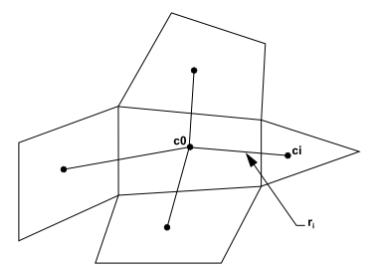
\includegraphics[width=0.5\textwidth]{foto02-minimos-quadrados.png}
	\caption[Avaliação do gradiente do volume de controle]{Avaliação do gradiente do volume de controle \cite{fluent2021ansys}.}
	\label{fig:minimos-quadrados}
\end{figure}
 
\subsubsection{Esquema QUICK}

O esquema QUICK \cite{Leonard1990} se baseia em uma média ponderada entre os esquemas \textit{upwind} de 2ª ordem (UDS-2) e diferenças centradas (CDS). Para um problema em 1-D, temos a \autoref{fig:ansys-QUICK} para explicar a lógica por trás dessa interpolação da seguinte forma (vide equação \ref{eq:esquema-quick}):

\begin{equation}
	\label{eq:esquema-quick}
	\phi_e = \theta\left[\frac{S_d}{S_c+S_d}\phi_P + \frac{S_c}{S_c+S_d}\phi_E \right] + (1 - \theta)\left[\frac{S_u+2S_c}{S_u+S_c}\phi_P - \frac{S_c}{S_c+S_u}\phi_W \right]
\end{equation}

\begin{figure}[!ht]
	\centering
	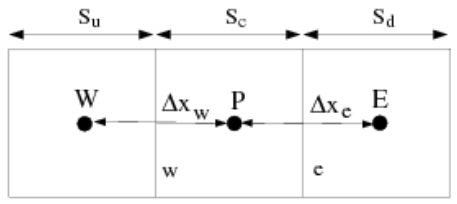
\includegraphics[width=0.5\textwidth]{foto03-quick-1d.png}  
	\caption[Esquema QUICK para um escoamento unidimensional.]{Esquema QUICK para um escoamento unidimensional \cite{fluent2021ansys}.}
	\label{fig:ansys-QUICK}
\end{figure}

A equação acima resulta no esquema CDS quando $\theta = 1$ e no UDS-2 quando $\theta = 0$. A versão tradicional do QUICK \cite{Leonard1979} considera $\theta = 1/8$. Comparado aos esquemas \textit{upwind} de 1ª ordem e diferenças centrais, é um modelo mais eficiente. A falsa difusão é baixa, mas deve-se levar em consideração de desvios nos resultados quando a geometria do problema for complexa \cite{Leonard1979}.

\subsection{Relaxação dos termos de alta ordem}

A proposta da relaxação é melhorar a inicialização e o comportamento da solução geral das simulações do escoamento quando discretizações espaciais de ordem superior são utilizadas (acima de 1ª ordem) \cite{fluent2021ansys}. A sub-relaxação desses termos segue a equação \ref{eq:relaxacao-altaordem} para qualquer propriedade $\phi$:

\begin{equation}
    \label{eq:relaxacao-altaordem}
    \phi_{novo} = \phi_{velho} + f(\phi_{novo} - \phi_{velho})
\end{equation}

Considera-se como padrão $f = 0,25$ em regime estacionário, foco deste presente trabalho.

\subsection{Método Multigrid}

O método \textit{Multigrid} \cite{Hutchinson1986} é usado no software desta pesquisa porque acelera a convergência através de uma sequência de correções em uma série de níveis de refino da malha. É um método bom para remover erros locais (alta frequência) e menos efetivo em erros globais (baixa frequência). Logo, o aumento no número de volumes de controle diminui o desempenho da técnica.

O \textit{Multigrid} é bastante eficiente quando se trata do esquema \textit{density-based} para remover os erros de alta frequência. Ele trabalha com uma sequência de malhas $M_1$ até $M_n$, cada vez mais grossas, onde o erro pode ser suavizado. Considerando um sistema linear do seguinte tipo:

\begin{equation}
    \label{eq:sistema-linear-multigrid}
    N_{ref}\phi + c = d
\end{equation}

Sendo $d$ um erro associado à solução aproximada $\phi$. Assumindo que $\phi_{ex} = \phi + \Psi$, onde $\phi_{ex}$ seria a solução exata e $\Psi$ um fator de correção do sistema linear acima \ref{eq:sistema-linear-multigrid}:

\begin{subequations}\label{eq:multigrid-corrigido} 
\begin{align}
    N_{ref}(\phi + \Psi) + b &= 0 \\
    \Psi + (N_{ref}\phi + b) &= 0 \\
    N_{ref}\Psi + d &= 0
\end{align}
\end{subequations}

A equação \ref{eq:multigrid-corrigido} serve para corrigir o operador original de nível de refino de malha $N_{ref}$ e o defeito $d$. Em cada etapa o valor de $\Psi$ será amortecido pelo esquema de relaxação e cada vez mais efetivo na próxima malha mais grosseira.

\subsection{Critério de Convergência}

O resíduo normalizado $R^{\phi}$ da equação de transporte discretizada é calculado a partir da equação \ref{eq:forma-linear-mvf} \cite{Rezende2009}:

\begin{equation}
\label{eq:criterio-convergencia}
	R^{\phi} = \frac{\sum_{células} \left[ \sum_{nb}a_{nb}\phi_{nb}+b-a_{P}\phi_{P}\right]}{\sum_{células}\left[a_{P}\phi_{P}\right]}    
\end{equation}

Assume-se que a solução está convergida quando $R^{\phi} < 10^{-6}$.